\chapterimage{chapter_head_2.pdf} % Chapter heading image

\chapter{Introdução}
%%%%%%%%%%%%%%%%%%%%%%%%%%%%%%%%%%%%%%%%%%%%%%%%%%%%%%%%%%%%%%%%%%%%%%%%%%%%%%%%
%% SECTION
%%%%%%%%%%%%%%%%%%%%%%%%%%%%%%%%%%%%%%%%%%%%%%%%%%%%%%%%%%%%%%%%%%%%%%%%%%%%%%%%
\section{Historia da samba}\index{historia da samba}
O samba é uns dos gêneros musicais mais conhecidos no Brasil do século XXI,
entre estes gêneros mais populares temos por exemplo o ``forró'' e o ``Sertanejo'';
sendo que o samba se distingue entre eles, 
como a principal expressão popular da música brasileira \cite[pp. 47]{diniz2008almanaque}. 


%O gênero samba atual é uma mistura de muitos gêneros musicais de África, América e Europa.
Porem, o caminho da palavra samba inicia muito tempo atras.
Nos inicios do seculo XIX os viajantes portugueses designavam as danças africanas com a palavra ``batuque'' \cite[pp. 54]{de4danccas},
e no Brasil existem registros desta palavra desde o século XVIII \cite[pp. 85]{sandroni2001feitico} , sendo que
esta não se usava para referenciar a uma dança em particular e sim aos festejos dos negros em geral.
Assim, a designação  ``batuque'' foi muito popular ate inícios do seculo XX, 
onde a palavra ``samba'' virou mais popular para descrever estes festejos \cite[pp. 85]{sandroni2001feitico} \cite[pp. 47]{diniz2008almanaque}; 
a Figura \ref{fig:sambacrono} descreve o uso destas palavras ao longo do tempo.
\begin{figure}[h]
  \centering
    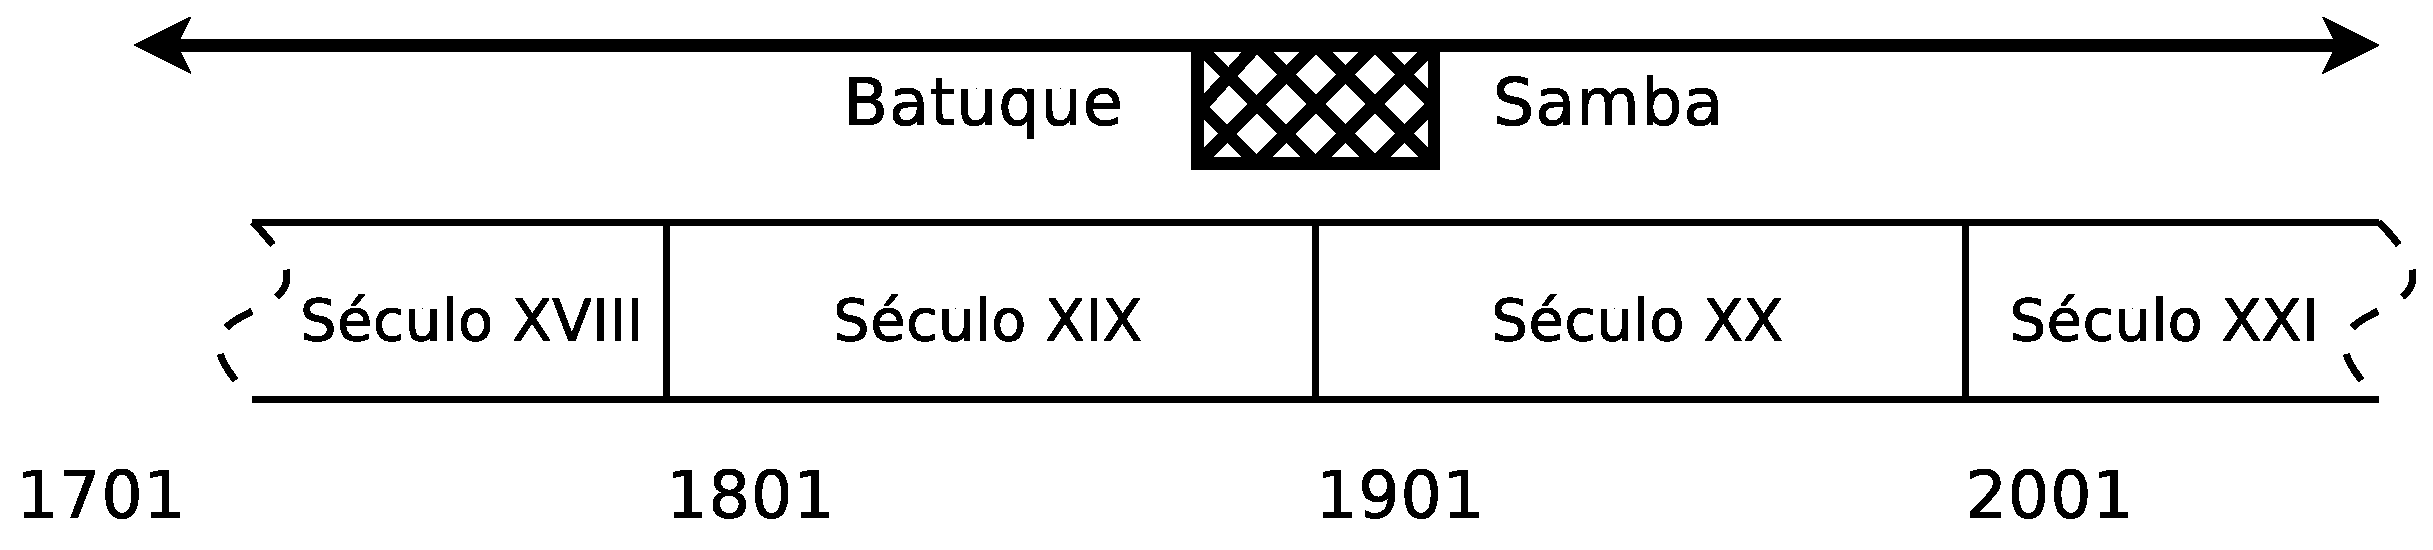
\includegraphics[width=0.85\textwidth]{chapters/cap-intro/samba-crono.eps}
  \caption{Cronologia da designação geral das danças africanas no Brasil.}
  \label{fig:sambacrono}
\end{figure}

Na literatura latino-americana a palavra ``samba'' é conhecida desde o seculo XIX, 
e no brasil desde o ano de 1838 \cite[pp. 47]{diniz2008almanaque}; porem , a palavra ``samba'' foi
quase desconhecida (em Rio de Janeiro) ate o último quartel do século XIX  \cite[pp. 86]{sandroni2001feitico}.
Entre as explicações da origem da palavra ``samba'', 
a mais conhecida, é a que promove que esta vem do idioma quimbundo, 
sendo derivado da palavra ``semba''  que significa umbigada \cite[pp. 47]{diniz2008almanaque} \cite[pp. 50]{da2015historia}.
Uma referencia muito conhecida deste vinculo é a descrita no livro ``O negro e o garimpo em Minas Gerais''
de Mata Machado Filho, onde ele comenta que ``os negros corrigem para semba se 
alguém lhes fala em samba'' \cite[pp. 85]{sandroni2001feitico}. Assim se vê que existe
desde antanho uma relação entre as palavras, 
samba, semba e umbigada.

Entre as danças "profanas" \cite[pp. 85]{sandroni2001feitico} afro-brasileiras o gesto da umbigada é um elemento muito caraterístico,
de modo que em 1961 Edson Carneiro definiu e englobou as danças que realizam este 
gesto como ``samba-de-umbigada'' . Assim tradições 
musicais como o samba de roda, o jongo, o lundu, o coco, o calango e o cateretê, 
seguindo Edson são englobadas com  ``samba-de-umbigada'' \cite[pp. 85]{sandroni2001feitico}.

%%%%%%%%%%%%%%%%%%%%%%%%%%%%%%%%%%%%%%%%%%%%%%%%%%%%%%%%%%%%%%%%%%%%%%%%%%%%%%%%
%% SECTION
%%%%%%%%%%%%%%%%%%%%%%%%%%%%%%%%%%%%%%%%%%%%%%%%%%%%%%%%%%%%%%%%%%%%%%%%%%%%%%%%
\section{Historia da música do samba}\index{música do samba}

\textcolor{red}{Pelo telefone}

%%%%%%%%%%%%%%%%%%%%%%%%%%%%%%%%%%%%%%%%%%%%%%%%%%%%%%%%%%%%%%%%%%%%%%%%%%%%%%%%
%% SECTION
%%%%%%%%%%%%%%%%%%%%%%%%%%%%%%%%%%%%%%%%%%%%%%%%%%%%%%%%%%%%%%%%%%%%%%%%%%%%%%%%
\section{Historia das gafieiras}\index{historia das gafieiras}




Desde inícios do século XX já existiam associações para negros e mestiços, 
com distintas  finalidades, entre elas estava a criação de 
"sociedades dançantes ou recreativas", abertas a um publico geral
\cite[pp. 154-155]{neres1999negro} \cite[pp. 71]{de2008bexiga} \cite[pp. 11]{respeitojournalbrasil1}.
Estas associações geralmente não tinham local próprio, 
e tinham que alugar espaços que terminavam sendo salões de velhos sobrados
ou similares \cite[pp. 154-155]{neres1999negro} \cite[pp. 49]{diniz2003almanaque}.

A primeira sociedade de dança, que agora definiriamos como gafieira, 
foi a ``Sociedade de Danças Clovis Invencivel'', 
fundado no Rio de Janeiro em 1906, 
onde eram populares concursos de valsa, polka ou quadrilha \cite[pp. 3]{entrevistajuliojournalbrasil1}.
A ideia da criação deste lugar de dança foi de um muito jovem, Júlio Simões,
que a seus 16 anos pensou numa sociedade de dança diferente dos da epoca,
dedicadas a ``bater bumbo'' (bailes carnavalescos), 
a uma dedicada a ``arrasta-pés'' (bailes de salão) \cite[pp. 3]{entrevistajuliojournalbrasil1}.

Com o surgir dos lugares de dança, 
Júlio Simões, e sócios, decidiram em 1914 fundar a ``Kanaga do Japão'',
lugar de grande tradição no Rio de Janeiro,
onde o conjunto encarregado de animar o local era cheifado por Sinhô e Bulhões de Carvalho,
que receberam o título popular de ``reis da valsa'',
com torneios de dança que duravam ate 55 minutos dançando uma valsa rápida \cite[pp. 3]{entrevistajuliojournalbrasil1}
\footnote{Informação extraída de uma entrevistas a Júlio Simões realizada o 3 de Agosto de 1961, no Jornal do Brasil.}.

Para o ano 1930, estas sociedades dançantes tinham ganhado muita popularidade, e salões de dança como a
"Kananga do Japão" eram dos mais concorridos. Porem,
apos a morte de um socio da "Kananga do Japão", 
Júlio Simões se associa com Heitor Persegani, e convida para ajudá-los a Hilário Jovino, 
e decidem fundar o local de danças chamado "Elite club" \cite[pp. 11]{eliteinaugura},
agora chamado "Elite clube" \cite[pp. 3]{juliosimoes},
na Rua Frei Caneca n. 4 - Centro, Rio de Janeiro - RJ;
sendo o 17 de julho de 1930 seu baile inaugural 
\cite[pp. 11]{eliteinaugura} \cite[pp. 3]{juliosimoes} \cite[pp. 10]{simoesjournalbrasil1}.

Uma descrição de uma destas sociedades dançantes, pode ser vista no livro "O cabrocha"; 
escrita  por Jota Efegê em 1931; 
sobre a "Sociedade Recreativa Familiar Bohemios de Botafogo" [pp. 24-26]\cite{jotaefege},
a continuação é mostrado um extracto desse texto:
\begin{tcolorbox}[colback=lowgray,colframe=lowgray]%%
O salão, comquanto não fosse de grandes dimensões, era
de um tamanho regular, confinando com uma pequena saleta
onde tambem se dansava; estava bem affluido. Numa
heterogeneidade foliã, via-se desde a crioulinha blasée, sem
elegancia, desalinhada, á mulatinha pernostica de faces
avermelhadas por um carmin berrante, cabello engommado e
subjugado por travessas e grampos, num á la garçonne
forçado, mas exigido pela moda. Em meio dessas "cabrochas"
e "roxinhas", viam-se algumas moças brancas de apparencia
sobria. São as meninas que não podem fazer um vestido de
seda ou calçar sapatos de setim, para se apresentarem no
Fluminense ou no Flamengo e que nestes clubes se divertem,
ficando em evidencia por serem brancas.
~\\
(Jota Efegê)
\end{tcolorbox}

O aparecimento do samba, 
foi um grande impacto para as pessoas que frequentavam estes já existosos lugares de dança;
sendo considerado um ritmo novo e ligeiro,
que desagradou aos bailarinos de maior idade e menos ágeis \cite[pp. 3]{entrevistajuliojournalbrasil1}.
O senhor, Júlio Simões chegou a temer pelo futuro da ``Kananga do Japão'' e
do ``Elite Club''; porem, para sorte dele, 
o samba fez muito sucesso no Elite,
e passou a ser considerado matéria indispensável para qualquer pessoa que pretendesse ser bailarino, 
compositor ou instrumentista \cite[pp. 3]{entrevistajuliojournalbrasil1}.

~\\

\textcolor{red}{``Aparece pela primeira vez no Jornal do Brasil a palavra gafieira. 
O titular da coluna Picareta, 
foi barrado pelos fiscais de Simões por estar em magas de camisa, ...
no dia seguinte escreveu: Aquele é um lugar de ralé, onde se cometem gafes em fieiras.'' \cite[pp. 188]{raca1999}.}

~\\

O termo gafieira foi criado pelo cronista carnavalesco, 
Romeu Arêde \footnote{Em algumas versões está mal referenciado como Romeu Aredo \cite[pp. 188]{raca1999}.}, 
também conhecido como "Picareta" \cite[pp. 18]{entrevistajuliojournalbrasil1} \cite[pp. 3]{juliosimoes} \cite[pp. 21]{efege1974maxixe} \cite[pp. 78]{coutinho2006cronistas}.

Devido a la denominação pejorativa de chamar a seu local um lugar de "gafes",
Júlio simões decide, em tom de zombaria, renomear seu local como "Gafieira Elite Clube" \cite[pp. 79]{moura1995tia},
sendo considerado por este fato a primeira gafieira do Brasil \cite{cabral2016elisete} \cite[pp. 84]{cabral1996escolas}.
Consequentemente, e em palavras de Jota Efegê, 
se considera a Júlio simões como o criador das gafieiras \cite[pp. 3]{juliosimoes}.

Nesse ponto da historia, 
o nome "gafieira" cobrou muita relevância e locais de dança apelidados como gafieiras surgiram no Rio de Janeiro;
depois de tudo, já existissem lugares com estas caraterísticas desde inícios do século XX \cite[pp. 49]{diniz2003almanaque}.
Os salões foram criadas a semelhança dos bailes de salão da classe média ou alta \cite[pp. 78]{coutinho2006cronistas}; 
porem, no caso das gafieiras, estas eram abertas ao público prévio pago da entrada.
A Figura \ref{fig:gafieiracrono} mostra a cronologia do uso da palavra gafieira para os salões de dança no Rio de Janeiro.
\begin{figure}[h]
  \centering
    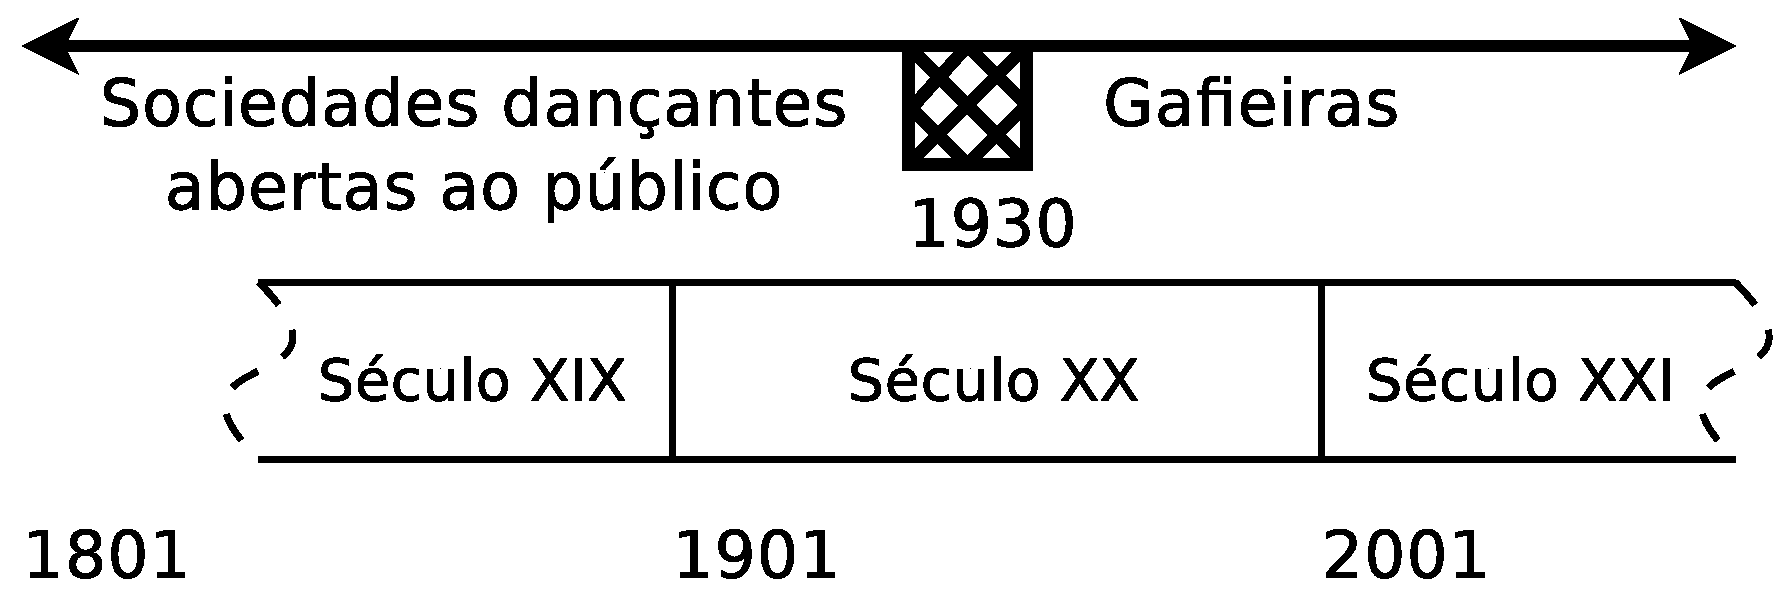
\includegraphics[width=0.65\textwidth]{chapters/cap-intro/gafieira-crono.eps}
  \caption{Cronologia da designação de gafieira para os salões de dança no Rio de Janeiro.}
  \label{fig:gafieiracrono}
\end{figure}

A primeira vez\footnote{Primeira coincidência achada na Biblioteca Digital da Fundação Biblioteca Nacional.} 
que o jornal ``O Radical'' (RJ) usa o neologismo ``gafieira'' 
é o dia 8 de setembro de 1932 \cite[pp. 12]{gafieirajournaloradical1},
com o titular:
\begin{tcolorbox}[colback=lowgray,colframe=lowgray]%%
A sahida do baile: Por causa de Aracy, o estivador foi ferido á baia.\\
... Na rua Domingo Lopes, n. 243, em Madureira, está situado o club de dança Ideal, 
conhecido pelos moradores locaes por ``Gafieira''.
\end{tcolorbox} 
Ao dia seguinte, 9 de setembro de 1932, o jornal ``A Batalha'' (RJ), 
usava também a palavra ``gafieira'' para se referir ao mesmo incidente \cite[pp. 8]{gafieirajournalabatalha1}.

O ``Jornal do Brasil'', o dia 9 de janeiro de 1934, 
usa também a palavra gafieira \cite[pp. 11]{gafieirajournalbrasil1}, com o titular:
\begin{tcolorbox}[colback=lowgray,colframe=lowgray]%%
À porta de uma ``gafieira''.
Ainda o conflito da madrugada de domingo no largo de Madureira.
Faleceu um dos soldados no Hospital da Policia Militar. 
Ha no largo de Madureira uma sociedade dansante, mais conhecida por ``gafieira'', 
com entradas retribuidas, ondem de quando em quando, se registram conflitos, 
alguns de graves consequências...
\end{tcolorbox} 
Como é visto nas refecerias dos jornais, 
o termo gafieira, estava associado a lugares um pouco perigosos;
isto propiciado pelo aumento do número de locais que se atribuíam este nome e a diversidade do seu público.
Porem, este não seria o padrão pelo qual se regiam todas as gafieiras, 
e certamente a conotação mais perigosa ou pejorativa iria mudando no tempo. 


Por exemplo, sobre o Elite Club,  nos sabemos que funcionava as quintas, sábados e domingos,
e existia um fiscal no salão (o velho Russo)\cite[pp. 37]{gafieirajournalmanchete}, 
que fazia cumprir estritamente as normas de bom-tom, comportamento social e respeito ao ambiente, como todo clube familiar precisa ter \cite[pp. 12]{respeitojournalbrasil1}; de modo que, 
não eram admitidas damas que não estivessem de sapatos de salto alto \cite[pp. 37]{gafieirajournalmanchete};
homens embriagados não entravam e o traje indispensável era o paletó e gravata, 
ou no mínimo camisa fechada \cite{entrevistajuliojournalbrasil1}.
O cavaleiro não podia abraçar a dama nem sentado na cadeira \cite{entrevistajuliojournalbrasil1},
né dançar de rosto colado, ou por a mão nas costas da dama sem usar lenço \cite[pp. 10]{simoesjournalbrasil1}, 
quem fiscalizava, na porta, era um preto velho tratado por todos de ``titio''  \cite[pp. 37]{gafieirajournalmanchete}.
Se alguma regra não era cumprida, o seu Júlio, jogava a qualquer um para fora \cite{entrevistajuliojournalbrasil1}.
Nos bailes dedicados ao padroeiro, todo 20 de janeiro, era obrigatório vestir de branco,
já seja no traje ou no vestido, incluindo sapatos e camisas \cite[pp. 37]{gafieirajournalmanchete}.
Tão grande era o censo de ordem dos frequentadores do Elite Club, 
que lhe era permitido operar estando a menos de 80 metros de um hospital,
sendo que nessa época existia a Lei n. 1.590 de 1924, 
seguindo a qual nenhuma casa de diversões podia estar a menos de 200 de estabelecimentos hospitalares,
Ate o proprio Delegado Dulcídio Gonçalves, da Delegacia de Costumes,
dispensava-se de mandar policiar o Elite.
``À casa do Júlio não precisa de policiamento'', dizia o Delegado Dulcídio
\cite[pp. 5]{simoesjournalalutademocratica1}.


Assim, ao transcorrer dos anos, essa visão popular mais obscura da palavra gafieira foi mudando;
pelo qual o jornalista Francisco Duarte, o dia 12 de agosto de 1979,
escreve no Jornal no Brasil (RJ) sobre este assunto com o título:
``Gafieira - Tratado geral do ambiente que exige respeito'' \cite{respeitojournalbrasil1},
explicando:
\begin{tcolorbox}[colback=lowgray,colframe=lowgray]%%
... o verbete Gafieira com o significado de baile reles, arrasta-pé, baile popular de baixa categoria.
No passado, encarada com má vontade pelos puristas do léxico e pela burguesia republicana dançante,
pode ter sido assim. Mas em 1979 -- e cabe aos dicionaristas verificar in loco --
gafieira é baile de clube particular, com entrada paga e freqüência livre, 
local de lazer e dança onde existe bom comportamento e muita compostura,
em perfeita integração racial.\\
(Francisco Duarte)
\end{tcolorbox} 
Além da afirmação anterior, 
o jornalista explica como a ``Delegacia de Diversões Públicas'' classifica as casas de dança;
onde temos: 
\begin{itemize}
\item ``boates'', que são bar restaurantes com pista de dança e palco para show;
\item ``cabarés'', onde se bebe, come, dança e se tem espetáculos de variedades;
\item ``dancings'' onde se dança mediante pagamento em cartões e picotes; e 
\item ``inferninhos'' que são boates de baixa categoria, 
frequentados por pessoas de vida irregular e onde se toca música barulhenta.
\end{itemize} 
Em palavras de Duarte, ``Gafieiras são sinônimos de baile em salão espaçoso como boa música orquestral'' \cite{respeitojournalbrasil1}.
%\textcolor{red}{A mudança de paradigma a ser agora um lugar de dança, com regras e entrada paga. }





%\newpage 
%%%%%%%%%%%%%%%%%%%%%%%%%%%%%%%%%%%%%%%%%%%%%%%%%%%%%%%%%%%%%%%%%%%%%%%%%%%%%%%%
%% SECTION
%%%%%%%%%%%%%%%%%%%%%%%%%%%%%%%%%%%%%%%%%%%%%%%%%%%%%%%%%%%%%%%%%%%%%%%%%%%%%%%%
\subsection{Estatutos da gafieira}\index{Estatuto da Gafieira}
Os "Estatutos da Gafieira" é uma composição musical escrita, por Billy Blanco;
esta foi interpretada por primeira vez na voz de Inezita Barroso, 
numa gravação da "RCA Victor" em janeiro de 1954 \cite{musicaestatuto};
O seguinte texto mostra a letra da música.
\begin{tcolorbox}[colback=lowgray,colframe=lowgray]%%
\center{Moço, olha o vexame,}\\
O ambiente exige respeito,\\
pelos estatutos da nossa gafieira,\\
dance a noite inteira, mas dance direito!\\
Aliás, pelo artigo 120,\\
o cavalheiro que fizer o seguinte:\\
subir na parede, dançar de pé pro ar,\\
morar na bebida sem querer pagar,\\
abusar da umbigada de maneira folgazã,\\
prejudicando hoje o bom crioulo de amanhã,\\
será distintamente censurado,\\
se balançar o corpo, vai pra mão do delegado.\\
Tá bem, moço?\\
\end{tcolorbox}
O texto é uma tentativa bem-humorada do autor de descrever o que acontecia 
nas gafieiras, porem na época da escrita desta popular samba, não
existiam tais estatutos\footnote{Estatutos, no sentido de regulamento, 
ordenança o conjunto de normas legais pelas que se regula o funcionamento de uma corporação ou associação.};
existia um código de costumes sim \cite[pp. 13]{respeitojournalbrasil1} em alguns salões, 
mas cada casa de dança imponia estes no seu local a critério do fiscal do salão ou donos \cite[pp. 10]{simoesjournalbrasil1} \cite{entrevistajuliojournalbrasil1} \cite[pp. 37]{gafieirajournalmanchete},
isto é confirmado por um depoimento realizado por 
Billy Blanco no 8 de julho de 2011 \cite{depoimentobilly}; o texto a seguir
mostra um fragmento dessa entrevista.

\begin{tcolorbox}[colback=lowgray,colframe=lowgray]%%
"Observando os acontecimentos de uma gafieira, então, eu imaginei
coisas, porque o compositor vive muito da imaginação. E eu criava situações 
possíveis de serem acontecidas na gafieira, ou então narrava o que
acontecia realmente. Por exemplo, no [samba] Pistom de Gafieira, tinha
um cidadão que era pistonista da orquestra que sempre tocava forte para
disfarçar quando a polícia vinha chegando. Doutra feita, eu tive a ideia
de fazer o estatuto para a gafieira. Então eu humorizei, porque ninguém
dança de pé pro ar, nem sobe em parede, não é? Mas a gente cria uma
extravagância dessas para dar uma certa graça, um certo sentido à música.
Na época, não havia código nenhum, eu apenas criei aquilo e muitas gafieiras 
depois tinham esse estatuto na parede para quem quisesse cantar.
Você vê que as regras do estatuto são umas regras brincalhonas, não é?" 
~\\
(Billy Blanco)
\end{tcolorbox}

Mesmo observando que as regras propostas pelo autor tem um caráter humorístico e sarcástico,
o texto foi adotado rapidamente pelas gafieiras, como um chamado a reflexão sobre umas
normas básicas a serem tidas em conta no salão, pois tem um alto grado de bom senso. Por exemplo: 
A linha 7, pode ser interpretada como uma indicação a 
não fazer movimentos aéreos na pista de dança,
ou  evitar movimentos capoerísticos; tudo isto
pelo evidente espacio reduzido e compartilhado que existe na pista de dança, 
além de que os movimentos aéreos estão pensados para ser
executados em apresentações e não em danças sociais. 
A linha 8, nos lembra o respeito ao parceiro; pois a pessoa que dança precisa
estar no controle de suas faculdades físicas e mentais; 
no caso dos condutores\footnote{\label{footlab:conducao}Nas danças sociais é comumente usado o paradigma da condução; 
onde no casal, uma pessoa assume o papel de condutor dos movimentos e 
a outra pessoa assume o papel de seguidor, este recebe a informação da condução e retorna uma resposta corporal.}, 
para estar atentos ao salão e cuidar do seu par enquanto os movimentos são executados, 
e no caso do seguidor\footref{footlab:conducao} para evitar problemas
nos giros e outros movimentos que precisem  controle do eixo do corpo.
As linhas 9 e 10 indicam sobre um conjunto de expressões artísticas 
afro-brasileiras emolduradas no século XIX com o nome de "samba umbigada" \cite[pp. 47]{diniz2008almanaque} \cite[pp. 85]{sandroni2001feitico}; nestas danças existe
um movimento chamado "umbigada" \cite{da2015historia} que da nome à dança, onde o ventre do homem e da mulher batem geralmente para indicar
a troca de dançarino; assim as linhas 9 e 10 se referem a
 evitar "abusar" de movimentos de umbigada que provem de danças que não eram bem vistas na época e eram consideradas gentílicas \cite[pp. 85]{sandroni2001feitico}.
Finalmente,
a linha 12 fala sobre balançar o corpo, que seguindo o contexto cultural, 
pode indicar não agir como bêbado\footnote{``Balançar o corpo; agitar, como o bebado, mal firme, e outros táes''-Diccionario da lingua portugueza, 1858.} \cite[pp.296]{diccionario1858}, ou em outras palavras,
com pouca elegância ou respeito,
caso contrario seria levado à delegacia!.


%\newpage 



%%%%%%%%%%%%%%%%%%%%%%%%%%%%%%%%%%%%%%%%%%%%%%%%%%%%%%%%%%%%%%%%%%%%%%%%%%%%%%%%
%% SECTION
%%%%%%%%%%%%%%%%%%%%%%%%%%%%%%%%%%%%%%%%%%%%%%%%%%%%%%%%%%%%%%%%%%%%%%%%%%%%%%%%
\section{Historia da samba de gafieira}\index{historia da samba de gafieira}


\textcolor{red}{Historia
\begin{description}
\item [A] Perna, Marco Antonio (2001). Samba de Gafieira - a história da dança de salão brasileira. ISBN 85-901965-5-0
\end{description}
}



